\documentclass[border=0pt]{standalone}
\usepackage{tikz}
\usetikzlibrary{calc,arrows.meta}

\definecolor{bgtop}{HTML}{070B1E}
\definecolor{bgbot}{HTML}{0E1A3F}
\definecolor{earth}{HTML}{0F3B6B}
\definecolor{earthhi}{HTML}{1D5FA0}
\definecolor{atmo}{HTML}{4FC3F7}
\definecolor{steel}{HTML}{B8C4D9}
\definecolor{solar}{HTML}{3B4FA8}
\definecolor{bA}{HTML}{38BDF8}
\definecolor{bB}{HTML}{F5A524}
\definecolor{bC}{HTML}{34D399}
\definecolor{bD}{HTML}{E879F9}
\definecolor{vel}{HTML}{FF6B81}

% \beam{x0}{y0}{x1}{y1}{color}: uplink lobe from a terminal toward the satellite
\newcommand{\beam}[5]{%
  \pgfmathsetmacro{\dx}{#3-#1}\pgfmathsetmacro{\dy}{#4-#2}%
  \pgfmathsetmacro{\ang}{atan2(\dy,\dx)}%
  \pgfmathsetmacro{\L}{sqrt(\dx*\dx+\dy*\dy)}%
  \pgfmathsetmacro{\w}{0.045*\L+0.06}%
  \begin{scope}[shift={(#1,#2)},rotate=\ang]
    \foreach \s/\o in {1.00/0.10, 0.62/0.17, 0.30/0.42}{
      \fill[#5,opacity=\o]
        (0,0) .. controls ({0.18*\L},{1.15*\w*\s}) and ({0.70*\L},{1.30*\w*\s}) .. (\L,0)
              .. controls ({0.70*\L},{-1.30*\w*\s}) and ({0.18*\L},{-1.15*\w*\s}) .. (0,0);
    }
    % wavefronts bunch up toward the satellite (Doppler)
    \foreach \t in {0.22,0.42,0.58,0.71,0.81,0.89}{
      \pgfmathsetmacro{\r}{\t*\L}\pgfmathsetmacro{\a}{atan(1.1*\w/\r)}
      \draw[#5,opacity=0.85,line width=0.8pt,line cap=round]
        ({\r*cos(-\a)},{\r*sin(-\a)}) arc[start angle=-\a,end angle=\a,radius=\r];
    }
  \end{scope}
}

% \terminal{x}{y}{color}: user terminal with a 2x2 dual-polarized array
\newcommand{\terminal}[3]{%
  \begin{scope}[shift={(#1,#2)}]
    \fill[#3,opacity=0.18] (0,0.15) circle (0.62);
    \fill[black!80,rounded corners=2pt,draw=#3,line width=1.1pt] (-0.34,-0.10) rectangle (0.34,0.42);
    \foreach \i in {0,1}{\foreach \j in {0,1}{
      \draw[#3,line width=0.9pt] ({-0.14+\i*0.28-0.07},{0.06+\j*0.21-0.07}) -- ++(0.14,0.14);
      \draw[#3,line width=0.9pt] ({-0.14+\i*0.28-0.07},{0.06+\j*0.21+0.07}) -- ++(0.14,-0.14);
    }}
    \draw[steel,line width=1pt] (0,-0.10) -- (0,-0.28);
  \end{scope}
}

\begin{document}
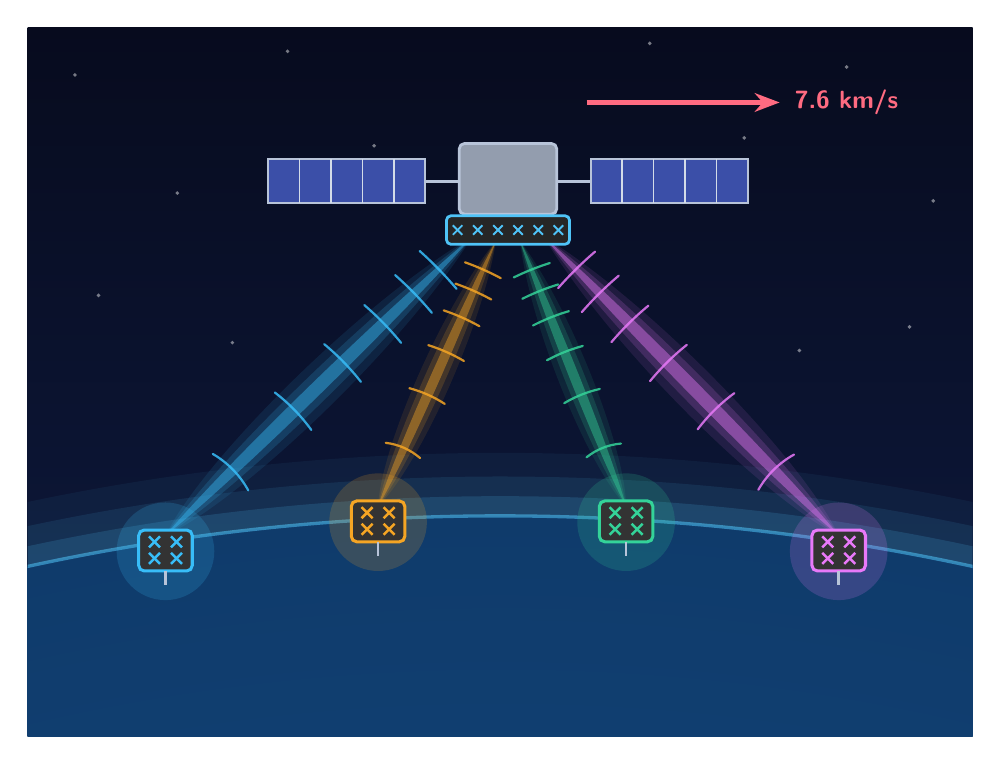
\begin{tikzpicture}
  \useasboundingbox (0,0) rectangle (12,9);
  \clip (0,0) rectangle (12,9);
  \shade[top color=bgtop,bottom color=bgbot] (0,0) rectangle (12,9);
  \foreach \x/\y in {0.6/8.4,1.9/6.9,3.3/8.7,4.4/7.5,7.9/8.8,9.1/7.6,10.4/8.5,11.5/6.8,0.9/5.6,11.2/5.2,2.6/5.0,9.8/4.9}{
    \fill[white,opacity=0.45] (\x,\y) circle (0.025);
  }

  % Earth with atmosphere glow
  \foreach \r/\o in {28.9/0.06,28.6/0.10,28.35/0.16}{\fill[atmo,opacity=\o] (6,-25.3) circle (\r);}
  \shade[inner color=earthhi,outer color=earth] (6,-25.3) circle (28.1);
  \draw[atmo,opacity=0.55,line width=1.2pt] (6,-25.3) circle (28.1);

  % uplink beams (terminals -> satellite array)
  \beam{1.75}{2.55}{5.65}{6.35}{bA}
  \beam{4.45}{2.92}{5.95}{6.30}{bB}
  \beam{7.60}{2.92}{6.25}{6.30}{bC}
  \beam{10.30}{2.55}{6.55}{6.35}{bD}

  % satellite
  \begin{scope}[shift={(6.10,7.05)}]
    \fill[solar,draw=steel,line width=0.8pt] (-3.05,-0.28) rectangle (-1.05,0.28);
    \fill[solar,draw=steel,line width=0.8pt] (1.05,-0.28) rectangle (3.05,0.28);
    \foreach \x in {-2.65,-2.25,-1.85,-1.45,1.45,1.85,2.25,2.65}{\draw[steel!60,line width=0.5pt] (\x,-0.28) -- (\x,0.28);}
    \draw[steel,line width=1.2pt] (-1.05,0) -- (-0.62,0) (0.62,0) -- (1.05,0);
    \fill[steel!80!black,rounded corners=2pt,draw=steel,line width=1pt] (-0.62,-0.42) rectangle (0.62,0.48);
    % dual-polarized planar array facing the ground
    \fill[black!85,draw=atmo,line width=1pt,rounded corners=1.5pt] (-0.78,-0.80) rectangle (0.78,-0.44);
    \foreach \i in {0,...,5}{
      \pgfmathsetmacro{\xx}{-0.64+\i*0.256}
      \draw[atmo,line width=0.7pt] (\xx-0.06,-0.68) -- (\xx+0.06,-0.56);
      \draw[atmo,line width=0.7pt] (\xx-0.06,-0.56) -- (\xx+0.06,-0.68);
    }
  \end{scope}
  % velocity arrow (Doppler)
  \draw[vel,line width=2pt,-{Stealth[length=9pt]}] (7.10,8.05) -- (9.55,8.05);
  \node[text=vel,font=\sffamily\bfseries\small,anchor=west] at (9.62,8.05) {7.6 km/s};

  % user terminals on the ground
  \terminal{1.75}{2.20}{bA}
  \terminal{4.45}{2.57}{bB}
  \terminal{7.60}{2.57}{bC}
  \terminal{10.30}{2.20}{bD}
\end{tikzpicture}
\end{document}
